
This analysis uses several different control regions in addition to the signal regions. 
All of these different regions are defined in this section. 
%Figure~\ref{fig:venndiagram} illustrates the relationship between these regions.

\subsection{Single Lepton Selection}

[UPDATE SELECTION]

The single lepton preselection sample is based on the following criteria, starting from the requirements described 
on \url{https://twiki.cern.ch/twiki/bin/viewauth/CMS/SUSYstop#SINGLE_LEPTON_CHANNEL}
\begin{itemize}
\item satisfy the trigger requirement (see
  Table.~\ref{tab:DatasetsData}). 
Note that the analysis triggers are inclusive single lepton triggers.
Dilepton triggers are used only for the dilepton control region.
\item select events with one high \pt\ electron or muon, requiring
  \begin{itemize}
  \item $\pt>30~\GeVc$  and $|\eta|<1.4442 (2.4)$ for electrons (muons)
  \item muon ID criteria is based on the 2012 POG recommended tight working point
  \item electron ID critera is based on the 2012 POG recommended medium working point
  \item PF-based isolation ($\Delta R < 0.3$, $\Delta\beta$ corrected) relative  $<$ 0.15 and absolute $<$ 5~GeV
  \item $|\pt(\rm{PF}_{lep}) - \pt(\rm{RECO}_{lep})| < 10~\GeV$
  \item $E/p_{in} < 4$ (electrons only)
  \end{itemize} 
  \item require at least 4 PF jets in the event with $\pt>30~\GeV$
    within $|\eta|<2.5$ out of which at least 1 satisfies the CSV
    medium working point b-tagging requirement
  \item require moderate $\met>50~\GeV$
\end{itemize}

%Table~\ref{tab:preselectionyield} shows the yields in data and MC without any corrections for this preselection region.

%\begin{table}[!h]
%\begin{center}
%\begin{tabular}{c|c}
%\hline
%\hline
%\end{tabular}
%\caption{  Raw Data and MC predictions without any corrections are shown after preselection. \label{tab:preselectionyield}}
%\end{center}
%\end{table}

\subsection{Signal Region Selection}

[MOTIVATIONAL BLURB ON MET AND MT, \\
CAN ADD SIGNAL VS. TTBAR MC PLOT \\
ADD SIGNAL YIELDS FOR AVAILABLE POINTS, \\
DISCUSS CHOICE SIG REGIONS]

The signal regions (SRs) are selected to improve the sensitivity for the
single lepton requirements and cover a range of scalar top
scenarios. The \mt\ and \met\ variables are used to define the signal
regions and the requirements are listed in Table~\ref{tab:srdef}. 

\begin{table}[!h]
\begin{center}
\begin{tabular}{l|c|c}
\hline
Signal Region & Minimum \mt\ [GeV] & Minimum \met\ [GeV] \\
\hline
\hline
SRA & 150 & 100 \\
SRB & 120 & 150 \\
SRC & 120 & 200 \\
SRD & 120 & 250 \\
SRE & 120 & 300 \\
\hline
\end{tabular}
\caption{ Signal region definitions based on \mt\ and \met\
  requirements. These requirements are applied in addition to the
  baseline single lepton selection.
\label{tab:srdef}}
\end{center}
\end{table}

Table~\ref{tab:srrawmcyields} shows the expected number of SM
background yields for the SRs. A few stop signal yields for four
values of the parameters are also shown for comparison. The signal
regions with looser requirements are sensitive to lower stop masses
M(\sctop), while those with tighter requirements are more sensitive to
higher M(\sctop). 

\begin{table}[!h]
\begin{center}
\begin{tabular}{l||c|c|c|c|c}
\hline
Sample              & SRA & SRB & SRC & SRD & SRE\\
\hline
\hline
\ttdl\ 		 & $619 \pm 9$& $366 \pm 7$& $127 \pm 4$& $44 \pm 2$& $17 \pm 1$ \\
\ttsl\ \& single top (1\Lep) 		 & $95 \pm 3$& $67 \pm 3$& $15 \pm 1$& $6 \pm 1$& $2 \pm 1$ \\
\wjets\ 		 & $29 \pm 2$& $15 \pm 2$& $6 \pm 1$& $3 \pm 1$& $1 \pm 0$ \\
Rare 		 & $59 \pm 3$& $38 \pm 3$& $16 \pm 2$& $8 \pm 1$& $4 \pm 1$ \\
\hline
Total 		 & $802 \pm 10$& $486 \pm 8$& $164 \pm 5$& $62 \pm 3$& $23 \pm 2$ \\
\hline
\end{tabular}
\caption{ Expected SM background contributions, including both muon
  and electron channels. This is ``dead reckoning'' MC with no
  correction.
It is meant only as a general guide. The uncertainties are statistical only. ADD
  SIGNAL POINTS.
\label{tab:srrawmcyields}}
\end{center}
\end{table}

\subsection{Control Region Selection}

[1 PARAGRAPH BLURB RELATING BACKGROUNDS (IN TABLE FROM PREVIOUS SECTION)
TO INTRODUCE CONTROL REGIONS]

Control regions (CRs) are used to validate the background estimation
procedure and derive systematic uncertainties for some
contributions. The CRs are selected to have similar
kinematics to the SRs, but have a different requirement in terms of
number of b-tags and number of leptons, thus enhancing them in
different SM contributions. The four CRs used in this analysis are
summarized in Table~\ref{tab:crdef}.

\begin{table}
\begin{center}
{\small
\begin{tabular}{l|c|c|c}
\hline
Selection 	& \multirow{2}{*}{exactly 1 lepton}	& \multirow{2}{*}{exactly 2
	leptons}		& \multirow{2}{*}{1 lepton + isolated
        track}\\
      Criteria & & & \\
\hline
\hline
\multirow{4}{*}{0 b-tags} 	 
& 	 CR1) W+Jets dominated:
& 	 CR2) apply \Z-mass constraint			 
& 	 CR3) not used \\  
& 	 
&       $\rightarrow$ Z+Jets dominated: Validate 
&      \\
&      Validate W+Jets \mt\ tail
& 	 \ttsl\ \mt\ tail comparing 
& 	 \\  
&
& 	 data vs. MC ``pseudo-\mt ''
& 	 \\  
\hline
\multirow{4}{*}{$\ge$ 1 b-tags} 	 
& 	
& 	CR4) Apply \Z-mass veto 
&      CR5) \ttdl, \ttlt\ and \\
&     SIGNAL 
&      $\rightarrow$ \ttdl\ dominated: Validate 
&	\ttlf\ dominated:  Validate \\
&     REGION 
&      ``physics'' modelling of \ttdl\     
&      \Tau\  and fake lepton modeling/\\
&
&
&      detector effects in \ttdl\     \\
\hline
\end{tabular}
}
\caption{Summary of signal and control regions.
  \label{tab:crdef}%\protect
}
\end{center}
\end{table}


\subsection{MC Corrections}

[UPDATE SECTION]

\subsubsection{Corrections to Jets and \met}

[UPDATE, ADD FEW MORE DETAILS ON WHAT IS DONE HERE]

The official recommendations from the Jet/MET group are used for 
the data and MC samples. In particular, the jet
energy corrections (JEC) are updated using the official recipe.
L1FastL2L3Residual (L1FastL2L3) corrections are applied for data (MC),
based on the global tags GR\_R\_42\_V23 (DESIGN42\_V17) for
data (MC). In addition, these jet energy corrections are propagated to
the \met\ calculation, following the official prescription for
deriving the Type I corrections. 

Events with anomalous ``rho'' pile-up corrections are excluded from the sample since these 
correspond to events with unphysically large \met\ and \mt\ tail
signal region. In addition, the recommended MET filters are applied. 


\subsubsection{Branching Fraction Correction}

The leptonic branching fraction used in some of the \ttbar\ MC samples
differs from the value listed in the PDG $(10.80 \pm 0.09)\%$. 
Table.~\ref{tab:wlepbf} summarizes the branching fractions used in
the generation of the various \ttbar\ MC samples. 
For \ttbar\ samples with the incorrect leptonic branching fraction, event
weights are applied based on the number of true leptons and the ratio
of the corrected and incorrect branching fractions. 

\begin{table}[!h]
\begin{center}
\begin{tabular}{c|c}
\hline
         \ttbar\ Sample - Event Generator & Leptonic Branching Fraction\\
\hline
\hline
Madgraph   &       0.111\\
MC@NLO    &       0.111\\
Pythia         &       0.108\\
Powheg       &       0.108\\
\hline
\end{tabular}
\caption{Leptonic branching fractions for the various \ttbar\ samples
  used in the analysis. The primary \ttbar\ MC sample produced with
  Madgraph has a branching fraction that is almost $3\%$ higher than
  the PDG value. \label{tab:wlepbf}}
\end{center}
\end{table}


\subsubsection{Lepton Selection Efficiency Measurements}

[TO BE UDPATED WITH T\&P STUDIES ON ID,ISO EFFICIENCIES]


\subsubsection{Trigger Efficiency Measurements}

In this section we measure the efficiencies of the single lepton triggers, HLT\_IsoMu24(\_eta2p1) for muons and HLT\_Ele27\_WP80 for electrons, using a tag-and-probe
approach. The tag is required to pass the full offline analysis selection and have \pt\ $>$ 30 GeV, $|\eta|<2.1$, and be matched to the single
lepton trigger. The probe is also required to pass the full offline analysis selection and have $|\eta|<2.1$, but the \pt\ requirement is relaxed to 20 GeV
in order to measure the \pt\ turn-on curve. The tag-probe pair is required to have opposite-sign and an invariant mass in the range 76--106 GeV.
The measured trigger efficiencies are displayed in Fig.~\ref{fig:trigeff} and summarized in Table~\ref{tab:mutriggeff} (muons) and Table~\ref{tab:eltriggeff} (electrons).
These trigger efficiencies will be applied to the MC when used to predict data yields selected by single lepton triggers. [THESE TRIGGER EFFICIENCIES TO BE APPLIED TO MC]


\begin{figure}[!ht]
\begin{center}
\begin{tabular}{cc}
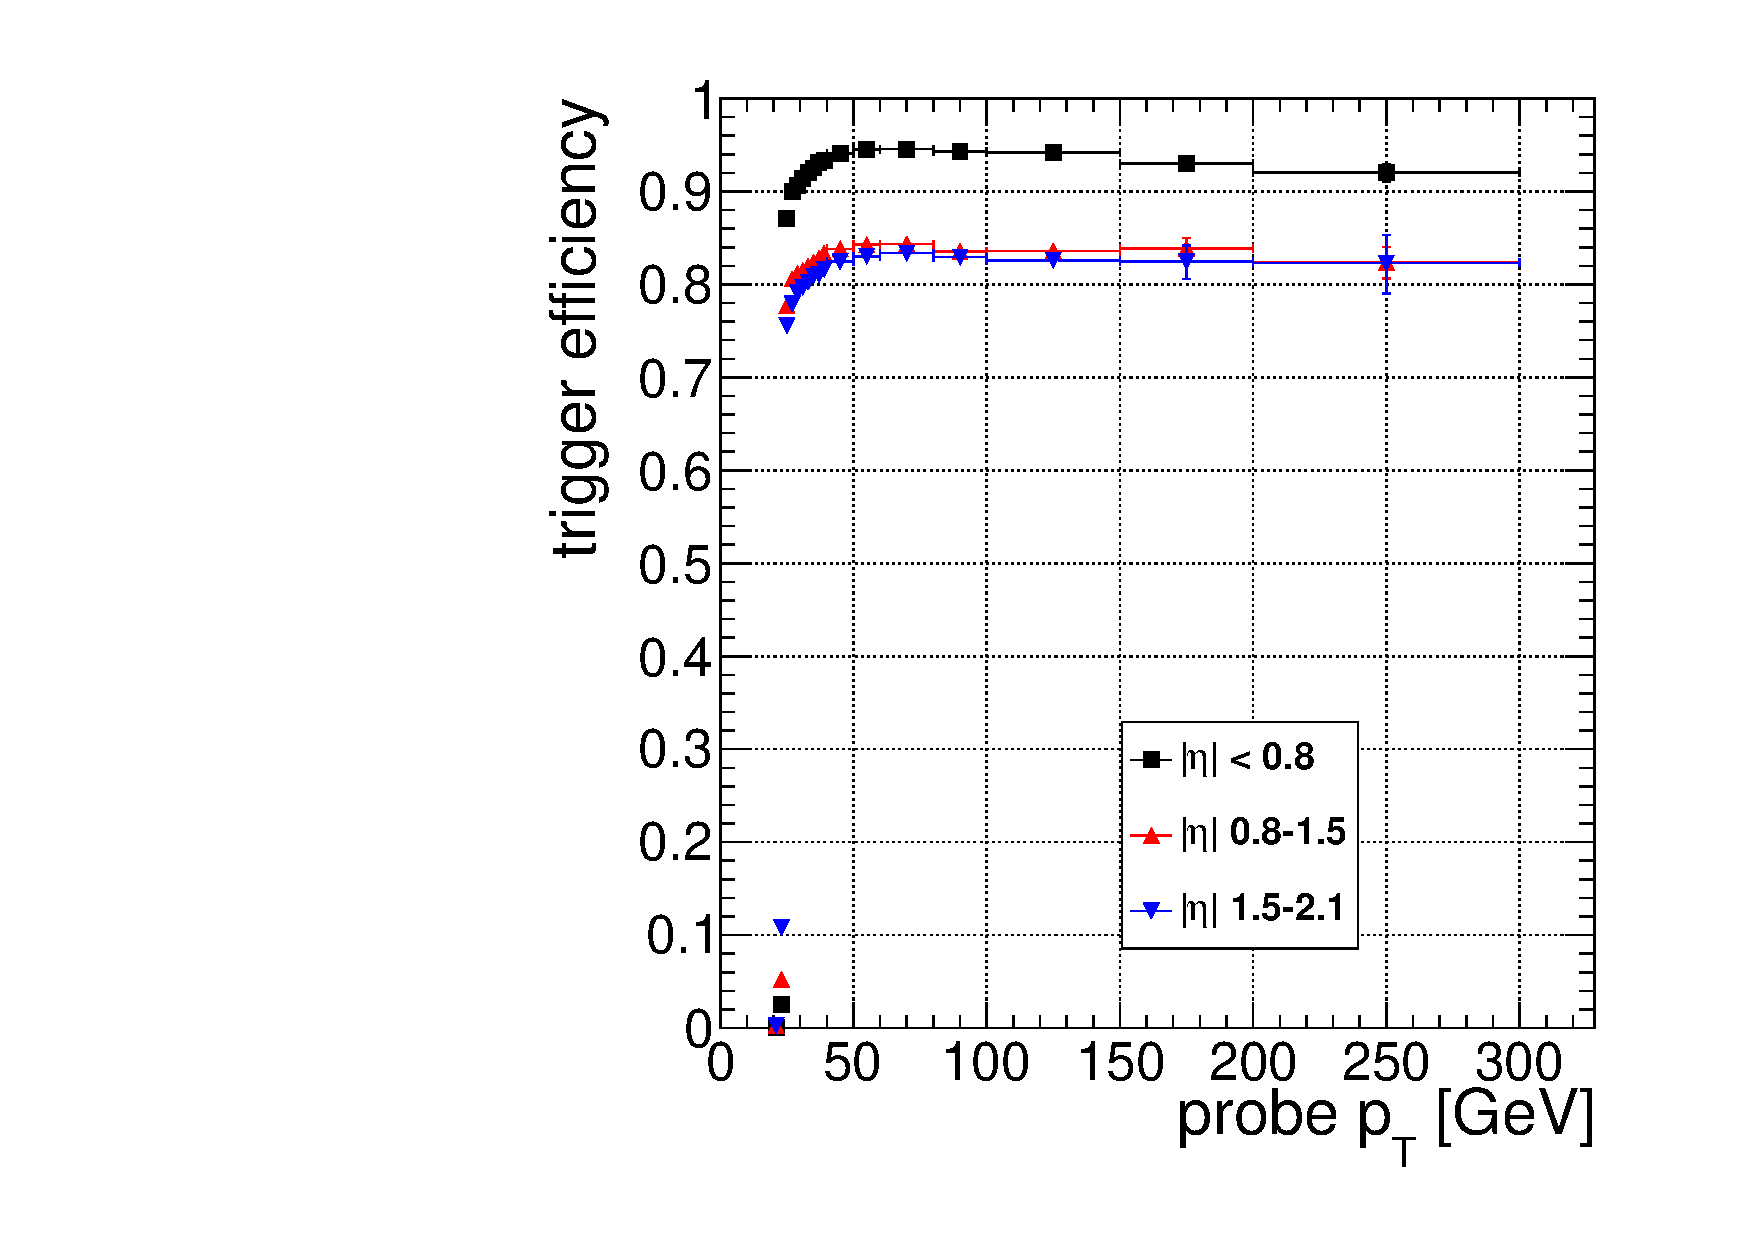
\includegraphics[width=0.4\textwidth]{plots/mutrig_pt_etabins.pdf} &
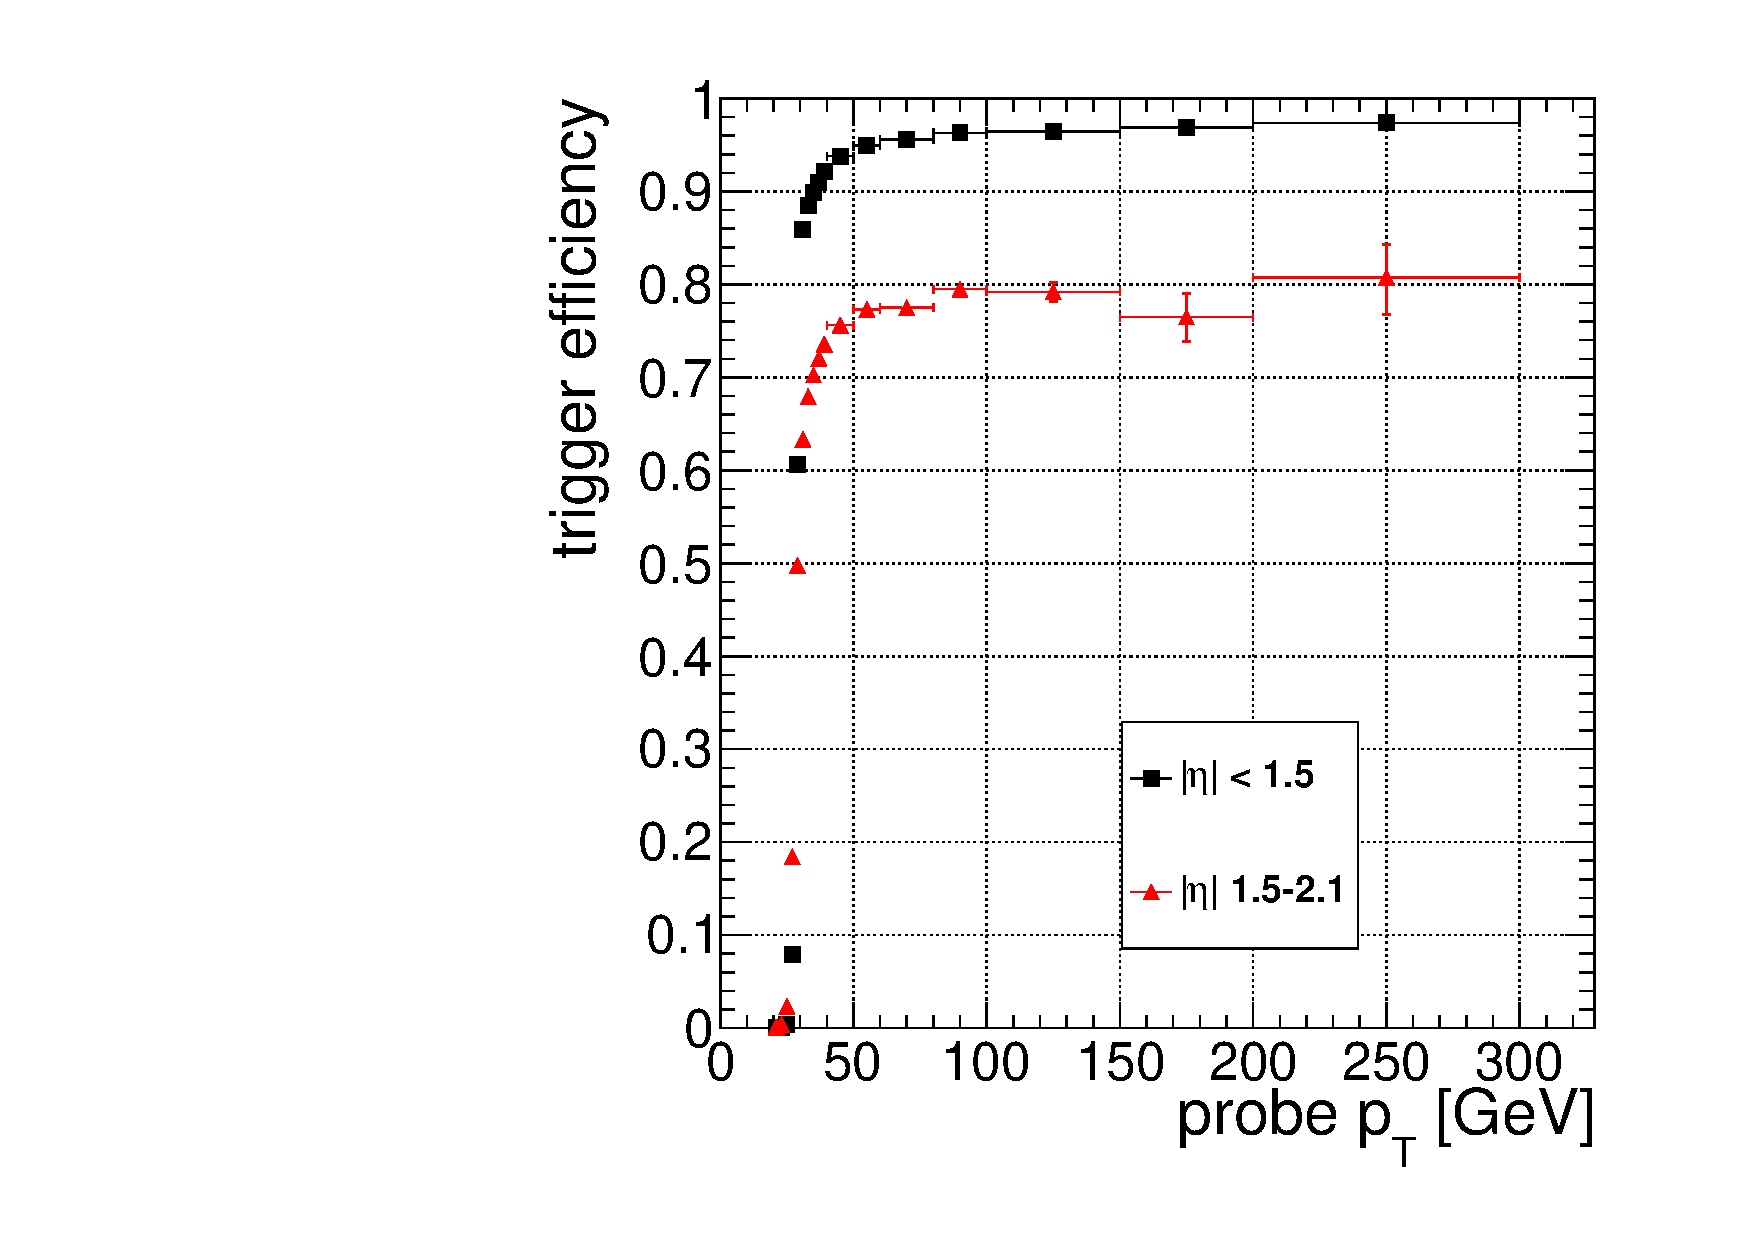
\includegraphics[width=0.4\textwidth]{plots/eltrig_pt_etabins.pdf} \\
\end{tabular}
\caption{\label{fig:trigeff}
Efficiency for the single muon trigger HLT\_IsoMu24(\_eta2p1) (left) and single electron trigger HLT\_Ele27\_WP80 (right) as a function of lepton \pt,
for several bins in lepton $|\eta|$.
}
\end{center}
\end{figure}

\clearpage

\begin{table}[htb]
\begin{center}
\footnotesize
\caption{\label{tab:mutriggeff}
Summary of the single muon trigger efficiency HLT\_IsoMu24(\_eta2p1). Uncertainties are statistical.}
\begin{tabular}{c|c|c|c}

\hline
\hline
  \pt\ range [GeV] & $|\eta|<0.8$ & $0.8<|\eta|<1.5$ & $1.5<|\eta|<2.1$ \\
\hline
  20 -  22  & 	0.00 $\pm$ 0.000 & 	0.00 $\pm$ 0.000 & 	0.00 $\pm$ 0.000 \\
  22 -  24  & 	0.03 $\pm$ 0.001 & 	0.05 $\pm$ 0.001 & 	0.11 $\pm$ 0.002 \\
  24 -  26  & 	0.87 $\pm$ 0.002 & 	0.78 $\pm$ 0.002 & 	0.76 $\pm$ 0.003 \\
  26 -  28  & 	0.90 $\pm$ 0.001 & 	0.81 $\pm$ 0.002 & 	0.78 $\pm$ 0.002 \\
  28 -  30  & 	0.91 $\pm$ 0.001 & 	0.81 $\pm$ 0.002 & 	0.79 $\pm$ 0.002 \\
  30 -  32  & 	0.91 $\pm$ 0.001 & 	0.81 $\pm$ 0.001 & 	0.80 $\pm$ 0.002 \\
  32 -  34  & 	0.92 $\pm$ 0.001 & 	0.82 $\pm$ 0.001 & 	0.80 $\pm$ 0.002 \\
  34 -  36  & 	0.93 $\pm$ 0.001 & 	0.82 $\pm$ 0.001 & 	0.81 $\pm$ 0.001 \\
  36 -  38  & 	0.93 $\pm$ 0.001 & 	0.83 $\pm$ 0.001 & 	0.81 $\pm$ 0.001 \\
  38 -  40  & 	0.93 $\pm$ 0.001 & 	0.83 $\pm$ 0.001 & 	0.82 $\pm$ 0.001 \\
  40 -  50  & 	0.94 $\pm$ 0.000 & 	0.84 $\pm$ 0.000 & 	0.82 $\pm$ 0.001 \\
  50 -  60  & 	0.95 $\pm$ 0.000 & 	0.84 $\pm$ 0.001 & 	0.83 $\pm$ 0.001 \\
  60 -  80  & 	0.95 $\pm$ 0.001 & 	0.84 $\pm$ 0.002 & 	0.83 $\pm$ 0.002 \\
  80 - 100  & 	0.94 $\pm$ 0.002 & 	0.84 $\pm$ 0.004 & 	0.83 $\pm$ 0.006 \\
 100 - 150  & 	0.94 $\pm$ 0.003 & 	0.84 $\pm$ 0.005 & 	0.83 $\pm$ 0.008 \\
 150 - 200  & 	0.93 $\pm$ 0.006 & 	0.84 $\pm$ 0.011 & 	0.82 $\pm$ 0.018 \\
 $>$200     & 	0.92 $\pm$ 0.010 & 	0.82 $\pm$ 0.017 & 	0.82 $\pm$ 0.031 \\
\hline
\hline

\end{tabular}
\end{center}
\end{table}

\begin{table}[htb]
\begin{center}
\footnotesize
\caption{\label{tab:eltriggeff}
Summary of the single electron trigger efficiency HLT\_Ele27\_WP80. Uncertainties are statistical.}
\begin{tabular}{c|c|c}

\hline
\hline
  \pt\ range [GeV] & $|\eta|<1.5$ & $1.5<|\eta|<2.1$ \\
\hline
  20 -  22   & 	0.00 $\pm$ 0.000 & 	0.00 $\pm$ 0.000 \\
  22 -  24   & 	0.00 $\pm$ 0.000 & 	0.00 $\pm$ 0.001 \\
  24 -  26   & 	0.00 $\pm$ 0.000 & 	0.02 $\pm$ 0.001 \\
  26 -  28   & 	0.08 $\pm$ 0.001 & 	0.18 $\pm$ 0.003 \\
  28 -  30   & 	0.61 $\pm$ 0.002 & 	0.50 $\pm$ 0.004 \\
  30 -  32   & 	0.86 $\pm$ 0.001 & 	0.63 $\pm$ 0.003 \\
  32 -  34   & 	0.88 $\pm$ 0.001 & 	0.68 $\pm$ 0.003 \\
  34 -  36   & 	0.90 $\pm$ 0.001 & 	0.70 $\pm$ 0.002 \\
  36 -  38   & 	0.91 $\pm$ 0.001 & 	0.72 $\pm$ 0.002 \\
  38 -  40   & 	0.92 $\pm$ 0.001 & 	0.74 $\pm$ 0.002 \\
  40 -  50   & 	0.94 $\pm$ 0.000 & 	0.76 $\pm$ 0.001 \\
  50 -  60   & 	0.95 $\pm$ 0.000 & 	0.77 $\pm$ 0.002 \\
  60 -  80   & 	0.96 $\pm$ 0.001 & 	0.78 $\pm$ 0.003 \\
  80 - 100   & 	0.96 $\pm$ 0.002 & 	0.80 $\pm$ 0.008 \\
  100 - 150  & 	0.96 $\pm$ 0.002 & 	0.79 $\pm$ 0.010 \\
  150 - 200  & 	0.97 $\pm$ 0.004 & 	0.76 $\pm$ 0.026 \\
$>$200       & 	0.97 $\pm$ 0.005 & 	0.81 $\pm$ 0.038 \\
\hline
\hline

\end{tabular}
\end{center}
\end{table}

\clearpage
